\chapter{Diseño e implementación} % Main chapter title
\label{Chapter3} % Change X to a consecutive number; for referencing this chapter elsewhere, use \ref{ChapterX}
En este capítulo se detalla cómo se ha ejecutado la implementación del trabajo,
incluyendo la arquitectura del sistema, procesamiento de peticiones,
modelos extensos de lenguaje utilizados y las técnicas empleadas sobre la inteligencia artificial.
Adicionalmente, se incluyen los hallazgos intermedios significativos que fueron fundamentales para la implementación final.

\definecolor{mygreen}{rgb}{0,0.6,0}
\definecolor{mygray}{rgb}{0.5,0.5,0.5}
\definecolor{mymauve}{rgb}{0.58,0,0.82}

%%%%%%%%%%%%%%%%%%%%%%%%%%%%%%%%%%%%%%%%%%%%%%%%%%%%%%%%%%%%%%%%%%%%%%%%%%%%%
% parámetros para configurar el formato del código en los entornos lstlisting
%%%%%%%%%%%%%%%%%%%%%%%%%%%%%%%%%%%%%%%%%%%%%%%%%%%%%%%%%%%%%%%%%%%%%%%%%%%%%
\lstset{ %
  backgroundcolor=\color{white},   % choose the background color; you must add \usepackage{color} or \usepackage{xcolor}
  basicstyle=\footnotesize,        % the size of the fonts that are used for the code
  breakatwhitespace=false,         % sets if automatic breaks should only happen at whitespace
  breaklines=true,                 % sets automatic line breaking
  captionpos=b,                    % sets the caption-position to bottom
  commentstyle=\color{mygreen},    % comment style
  deletekeywords={...},            % if you want to delete keywords from the given language
  %escapeinside={\%*}{*)},          % if you want to add LaTeX within your code
  %extendedchars=true,              % lets you use non-ASCII characters; for 8-bits encodings only, does not work with UTF-8
  %frame=single,	                % adds a frame around the code
  keepspaces=true,                 % keeps spaces in text, useful for keeping indentation of code (possibly needs columns=flexible)
  keywordstyle=\color{blue},       % keyword style
  language=[ANSI]C,                % the language of the code
  %otherkeywords={*,...},           % if you want to add more keywords to the set
  numbers=left,                    % where to put the line-numbers; possible values are (none, left, right)
  numbersep=5pt,                   % how far the line-numbers are from the code
  numberstyle=\tiny\color{mygray}, % the style that is used for the line-numbers
  rulecolor=\color{black},         % if not set, the frame-color may be changed on line-breaks within not-black text (e.g. comments (green here))
  showspaces=false,                % show spaces everywhere adding particular underscores; it overrides 'showstringspaces'
  showstringspaces=false,          % underline spaces within strings only
  showtabs=false,                  % show tabs within strings adding particular underscores
  stepnumber=1,                    % the step between two line-numbers. If it's 1, each line will be numbered
  stringstyle=\color{mymauve},     % string literal style
  tabsize=2,	                   % sets default tabsize to 2 spaces
  title=\lstname,                  % show the filename of files included with \lstinputlisting; also try caption instead of title
  morecomment=[s]{/*}{*/}
}


%----------------------------------------------------------------------------------------
%	SECTION 1
%----------------------------------------------------------------------------------------
\section{Arquitectura del sistema}

Los primeros esfuerzos en el desarrollo del trabajo se enfocaron en definir el conjunto de módulos que compondrían la solución.
Estos componentes fueron identificados correctamente desde el principio:
un servidor \textit{web} y un módulo de modelos extensos de lenguaje.
Sin embargo, su relación en el sistema sí cambió durante la fase de implementación.

Inicialmente, durante la fase de diseño, se concibió que el servidor \textit{web} también alojaría el modelo extenso de lenguaje 
y sería responsable de gestionar su conjunto de datos, entrenamiento y despliegue.
Esta decisión se tomó al principio de la implementación,
influenciada por la forma en la que se trabaja con redes neuronales sencillas.
Hacer que esa arquitectura funcionase en este trabajo era mucho más complejo de lo estimado
por la propia naturaleza de los modelos extensos de lenguaje.
La incertidumbre generada por la ausencia de un conjunto de datos de calidad y tamaño suficientes,
y la dificultad implícita de reentrenar un modelo tan grande,
fueron un factor de riesgo permanente durante la fase de diseño.

Fue necesario profundizar en las materias de procesamiento de lenguaje natural y \textit{Large Language Models} \cite{fiubaLlm}
para definir una solución efectiva a este problema.
Finalmente se decidió por no solo ``extraer'' el módulo de modelos extensos de lenguaje del servidor \textit{web}
sino por simplificar su complejidad de programación haciendo uso de la herramienta LM Studio.
Este programa permite administrar los modelos locales de la computadora,
añadir nuevos a través de una interfaz de descarga
y hacer uso del hardware disponible para arrancarlos de forma transparente para el usuario.
Además, cuenta con varias ventanas de configuración de parámetros de lanzamiento del modelo, \textit{prompts} personalizados,
salida estructurada a través de un esquema JSON,
opciones relacionadas con la aleatoriedad y temperatura de la inferencia y otras características experimentales.

De este modo, el servidor \textit{web} también se simplificó en el desarrollo, ahorró mucho trabajo de programación sin
comprometer la calidad del proceso de la inteligencia artificial.
Esto también es coherente con la arquitectura de servidor ligero esperable en un prototipo
y tiene una mejor sinergia con bibliotecas orientadas al despliegue de servidores sencillos.

Tal y como se muestra en la figura \ref{fig:sist},
el prototipo es accesible para los clientes a través del protocolo HTTP-REST que expone el servidor.
Además, durante el desarrollo se implementó una sencilla página \text{web} para realizar peticiones de prueba
y mostrar la salida de texto obtenida.

\begin{figure}[htbp]
	\centering
	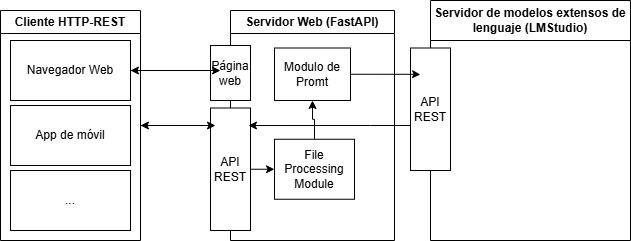
\includegraphics[width=0.9\textwidth]{./Figures/Sistema_es.png}
	\caption{Arquitectura del sistema.}
	\label{fig:sist}
\end{figure}

Otra ventaja de haber diseñado ambos módulos de forma independiente es que facilita al cliente
profundizar de forma paralela en los componentes sin comprometer el funcionamiento del resto del sistema.
Puede decidir si sustituir la implementación de uno u ambos módulos, escalarlos y distribuirlos en distintos entornos
para ajustarlo a su aplicación para \text{smartphones} y plan de expansión de servicios. 

%----------------------------------------------------------------------------------------
%	SECTION 2
%----------------------------------------------------------------------------------------
\section{Procesamiento de peticiones \textit{web} y ficheros}
Para la implementación del servidor web se decidió utilizar la biblioteca de FastAPI \cite{fastapi}.
Es una biblioteca moderna y de alto rendimiento para la construcción de APIs \text{web} en Python,
diseñada sobre estándares como OpenAPI \cite{openapi} y JSON schema.
Ofrece una forma rápida y eficiente de desarrollar interfaces REST
con una sintaxis sencilla y basada en anotaciones.
Esto permite una validación automática de datos de entrada y generación de documentación.
Todo esto hace que FastAPI sea una opción ideal para construir microservicios y prototipos rápidos.

El servidor expone dos servicios principales.
El primero es un \textit{endpoint} de tipo GET que proporciona la página \textit{web} que visualiza la interfaz gráfica del prototipo.
El otro servicio implementa un método POST para recibir las peticiones de consulta por parte del usuario para su procesamiento
y reenvío al módulo de inteligencia artificial. 


\pagebreak
\subsection{Procesamiento de peticiones}
En la figura \ref{fig:flux} se representa el diagrama de flujo correspondiente al manejo de las peticiones entrantes.

\begin{figure}[htbp]
	\centering
	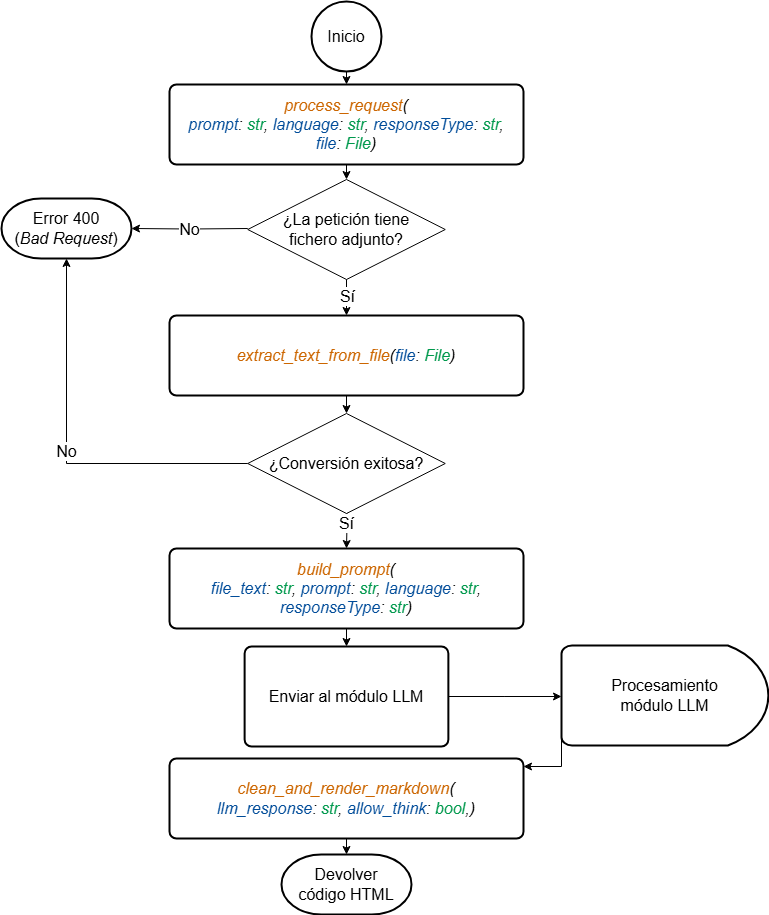
\includegraphics[width=1\textwidth]{./Figures/flux-diagram.png}
	\caption{Diagrama de flujo del procesamiento de peticiones.}
	\label{fig:flux}
\end{figure}

El proceso comienza cuando el cliente envía una solicitud con los datos de consulta a través de un cliente REST.
Esto puede ser a través del formulario proporcionado por el servidor o a través de cualquier otra herramienta como,
por ejemplo, PostMan.
Tras realizar las comprobaciones iniciales,
el servidor continúa procesando la información mediante una serie de funciones específicas:
\begin{itemize}
\item \texttt{extract\_text\_from\_file}:
es el proceso encargado de extraer la información textual de los ficheros adjunto
y formatearlo para que el módulo de modelos extensos de lenguaje sea capaz de interpretarlo.
En esta función se hace uso de las bibliotecas de cgardet, docx y fitz para la detección del formato y
su conversión a texto plano.
\item \texttt{build\_prompt}:
esta función es la encargada de construir el \textit{prompt} a partir del texto extraído del fichero
y las entradas adicionales proporcionadas por el usuario, entre las que se incluyen el idioma de
la respuesta, el tipo de listado que se solicita y algunas instrucciones adicionales.
En esta función se emplea la ingeniería de \textit{prompting} que se envía posteriormente al módulo LLM.
Se detalla más adelante en la sección \ref{subsec:prompt}.
\item \texttt{clean\_and\_render\_markdown}:
esta función se encarga de limpiar la salida y formatearla en código HTML
a través de la biblioteca markdown para una mejor legibilidad en navegadores web.
\end{itemize}

Cabe destacar que para la comunicación con el módulo LLM,
aunque LM Studio ofrece un SDK en Python para interactuar mediante programación,
se optó por utilizar su interfaz REST.
La razón es que así el servidor \textit{web} no depende exclusivamente de la biblioteca de LM Studio.
Al emplear un protocolo de comunicación estándar como REST,
el servidor web puede interactuar fácilmente con cualquier otro servicio que aloje modelos extensos de lenguaje,
lo que le da mayor flexibilidad.

\subsection{Interfaz gráfica}
El servidor también facilita el acceso a una página \textit{web} con la interfaz gráfica del prototipo,
tal y como se aprecia en la figura \ref{fig:webPage}.

\begin{figure}[htbp]
	\centering
	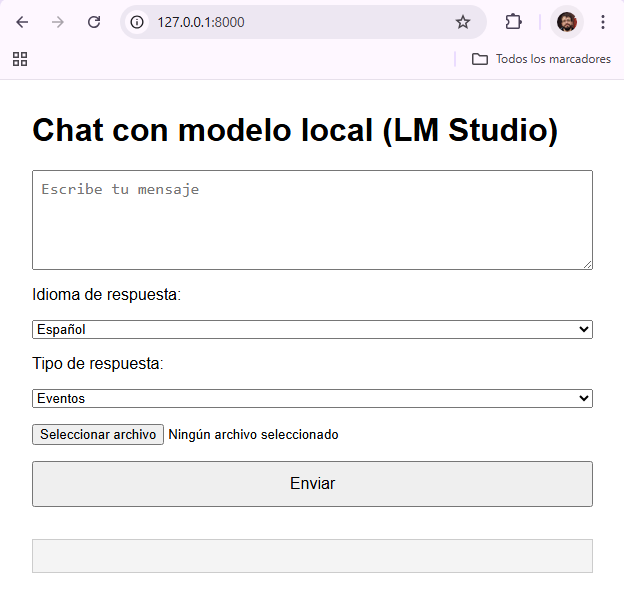
\includegraphics[width=0.8\textwidth]{./Figures/webpage.png}
	\caption{Interfaz gráfica del prototipo.}
	\label{fig:webPage}
\end{figure}

El formulario consta de los siguientes elementos:
\begin{itemize}
\item Cuadro de texto:
este elemento se utiliza para darle las instrucciones específicas a la inteligencia artificial.
Está pensado para que sea un mensaje breve y conciso que pueda ayudar al usuario a guiar un poco mejor la respuesta.
Es un parámetro opcional y puede dejarse en blanco.
\item Idioma de respuesta:
se trata de un \textit{combobox} que contiene dos opciones: inglés y español.
El módulo LLM responderá en el idioma seleccionado, independientemente del idioma del fichero de entrada.
Este elemento se añadió porque algunos modelos presentan comportamientos anómalos si responden en un idioma distinto al inglés.
\item Tipo de respuesta:
permite a la inteligencia artificial centrar su respuesta en un aspecto concreto de la narrativa.
Al estar instruida en devolver listas de elementos, la idea es que el usuario pueda elegir la opción
específica de la creación de mundos que le interese.
\item Fichero adjunto:
es el elemento más importante del formulario.
El usuario puede agregar un fichero con el contexto narrativo existente
y enviarlo a la inteligencia artificial para que genere nuevo contenido.
\end{itemize}

%----------------------------------------------------------------------------------------
%	SECTION 3
%----------------------------------------------------------------------------------------
\section{Gestión de modelos extensos de lenguaje}
El siguiente paso en la fase de implementación fue la instalación
y configuración del módulo de modelos extensos de lenguaje.
Inicialmente, se analizó si la gestión y comunicación con la LLM se haría a través de una
API en la nube o alojarlo localmente en el servidor \textit{web}.

La opción de la API implicaba depender de servicios externos
en internet, lo que resultaba en peores tiempos de respuesta y un coste adicional significativo
debido a los modelos de pago por uso que restringen la cantidad de consultas.
A su vez, la interacción con servicios externos exponía la información transmitida en las consultas
lo que podría incumplir los requerimientos de protección de la privacidad
y propiedad intelectual de los datos del cliente.
También se observó un menor número de modelos disponibles y opciones de personalización,
lo que dificultaba la experimentación y adaptación de los LLM a las necesidades específicas del sistema.

Por otra parte, la opción de gestionar los modelos extensos de lenguaje
de forma nativa presentaba desafíos considerables.
Desarrollar la infraestructura \textit{software} necesaria para la gestión de modelos
era una tarea con alta complejidad técnica que iba más allá de la mera integración de \textit{frameworks}.
Esto podía suponer limitaciones significativas en el proceso de configuración de los modelos y,
en consecuencia, provocar un coste elevado en términos de tiempo y recursos de desarrollo.

Por estos motivos se decidió buscar alternativas para este módulo y se encontraron varias herramientas que
cumplían con las características deseadas, y las más llamativas fueron
Ollama \cite{ollama}, GPT4All \cite{gpt4all} y LM Studio \cite{lmstudio}.
Esta última fue la opción elegida eventualmente por su interfaz intuitiva y buscador de modelos,
además de simplificar la gestión y configuración de los LLM.
Alojar localmente los modelos permite el envío ilimitado de consultas
y cumple con los requisitos de privacidad de los datos del cliente.

En los siguientes apartados se detallan los distintos procesos de gestión que se llevaron a cabo con LM Studio.

\subsection{Descarga de modelos}
El menú \textit{discover} de LM Studio da acceso al explorador de modelos extensos de lenguaje,
permitiendo a los usuarios navegar por una vasta biblioteca alojada principalmente en la plataforma Hugging Face \cite{huggingface}.
Como se ilustra en la figura \ref{fig:downloadMenu},
esta herramienta de búsqueda facilita la localización de modelos específicos mediante filtros por nombre o palabras clave,
presentando los resultados en un listado que se ajusta a los criterios definidos.
Al seleccionar un modelo, se muestra una sección de detalles con sus características y las distintas opciones de descarga disponibles.

\begin{figure}[htbp]
	\centering
	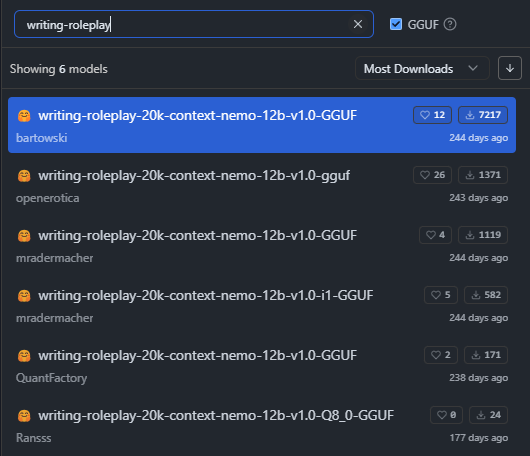
\includegraphics[width=0.8 \textwidth]{./Figures/download_menu.png}
	\caption{Buscador de modelos de LM Studio.}
	\label{fig:downloadMenu}
\end{figure}

Esta herramienta se empleó para la búsqueda y descarga de múltiples modelos,
que se enumeran y detallan en la subsección \ref{subsec:modelos-llm}.
Se eligieron tanto modelos generalistas como aquellos especializados en \textit{roleplay},
con el fin de analizar y comparar su rendimiento en tareas de construcción de mundos.

\subsection{Administración y configuración de modelos}
LM Studio permite la gestión y configuración de los modelos locales en el menú \textit{My Models}.
Además de listar los LLM descargados en el equipo, esta ventana permite personalizar
sus parámetros de ejecución para optimizar el rendimiento y la precisión de las respuestas.

\pagebreak
Como se muestra en la figura \ref{fig:configMenu},
al seleccionar un modelo se tiene acceso a un conjunto de ajustes agrupados
en varios conjuntos.
Como se trabajó en el \textit{prompting} en el servidor \textit{web},
los esfuerzos de configuración se centraron en los parámetros de carga e inferencia.

\begin{figure}[htbp]
	\centering
	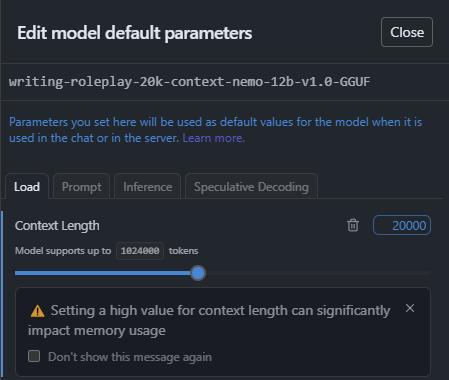
\includegraphics[width=0.8 \textwidth]{./Figures/config_menu.png}
	\caption{Configurador de modelos de LM Studio.}
	\label{fig:configMenu}
\end{figure}

La longitud del contexto resultó ser un parámetro fundamental en el trabajo.
Dado que las consultas de los usuarios se espera que vengan acompañadas de relatos extensos de \textit{worldbuilding},
era crucial que el LLM pudiera procesar y comprender grandes volúmenes de texto para generar respuestas coherentes y relevantes.
Los modelos tienen configurado por defecto un tamaño de contexto de 2048 o 4096 \textit{tokens},
un valor muy por debajo del tamaño de petición que se estima.

Para superar esta limitación, se seleccionó un tamaño de contexto compatible con las capacidades relativas de cada modelo,
a menudo indicado en los detalles.
Esta configuración fue esencial para asegurar que los LLM pudieran asimilar la totalidad de los relatos proporcionados.
Adicionalmente, se exploraron diversas tácticas para gestionar el exceso de contexto,
resultando más eficaces el acortamiento desde el principio de la secuencia o desde su punto medio.

Los parámetros de configuración de inferencia más importantes fueron la temperatura y
las técnicas de muestreo de probabilidad, como Top P o Top K.
Durante el desarrollo del proyecto, se observó que los valores predeterminados para estas variables
ya eran bastante adecuados. Por eso, solo fue necesario hacer ajustes mínimos en algunas de ellas.

Por defecto todos los modelos incluyen una sección de razonamiento.
Este parámetro fue deshabilitado en la configuración del modelo
y se filtró en el post-procesamiento para que no se mostrara en la respuesta al usuario.

\pagebreak
\subsection{Ejecución de modelos e interfaz REST}
La herramienta muestra y administra qué LLMs están activos y cargados en la memoria del sistema.
Además, también puede desplegar con un solo \textit{click} un servidor local compatible con la interfaz REST de OpenAI.
Cuando las peticiones llegan a este servidor, se registran en un log detallado que no solo proporciona
información sobre su estado sino que también muestra datos cruciales para la depuración de salidas incorrectas o errores.

\begin{figure}[htbp]
	\centering
	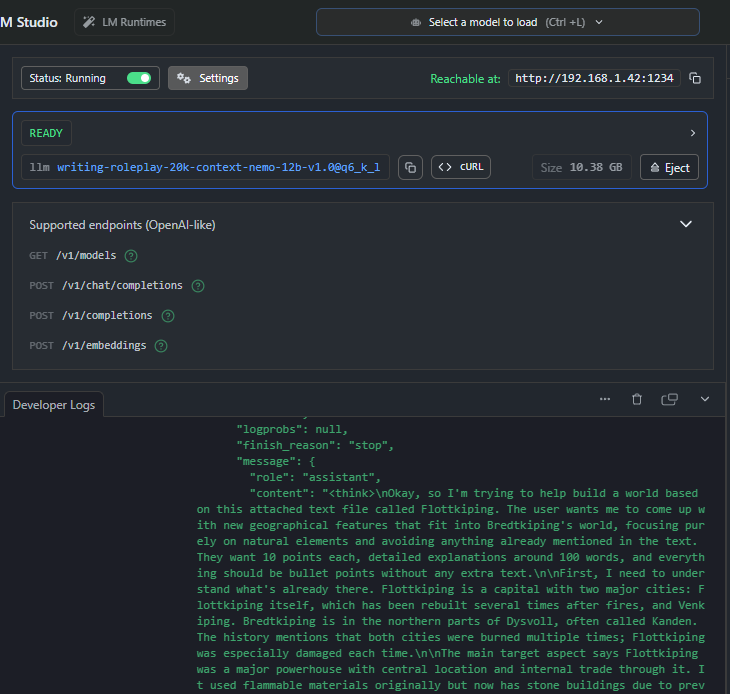
\includegraphics[width=1.0 \textwidth]{./Figures/developer_menu.png}
	\caption{Menú de desarrollador de LM Studio.}
	\label{fig:developerMenu}
\end{figure}

Una vez el modelo y el servidor están activos, el flujo del procesamiento de peticiones de la solución está completo.
El LLM, ya configurado con el tamaño de contexto ampliado y los parámetros de aleatoriedad ajustados,
gestiona la entrada, generando las respuestas esperadas.
Este diseño permite la misma forma de gestionar las peticiones,
sin importar el modelo que esté activo.

\pagebreak
\subsection{Modelos extensos de lenguaje utilizados}\label{subsec:modelos-llm}
El conjunto de modelos empleados en este trabajo se obtuvo a través de la herramienta de descarga de LM Studio.
Fueron seleccionados con un número de parámetros y un nivel de cuantización adecuado,
sin superar el límite de 12~GB de tamaño en memoria RAM dedicada en la tarjeta gráfica.
Esta parametrización permite aprovechar al máximo las capacidades del \textit{hardware} disponible,
con el objetivo de evaluar el rendimiento de distintos LLMs en tareas de generación narrativa.
En la tabla~\ref{tab:modelos_llm} se detallan las características de cada modelo:

\begin{table}[h]
\centering
\caption{Modelos extensos de lenguaje utilizados en el trabajo.}
\resizebox{\textwidth}{!}{%
\begin{tabular}{l l c c c r}
\toprule
\textbf{Modelo} & \textbf{Editor} & \textbf{Arquitectura} & \textbf{Parámetros} & \textbf{Cuantización} & \textbf{Tamaño (Contexto / VRAM)} \\
\midrule
\texttt{arliai-rpmax-v1.4} & bartowski & Mistral & 24 B & Q3\_K\_S & 20 k tokens / 10,40 GB \\
\texttt{writing-roleplay-v1.0} & bartowski & LLaMA & 12 B & Q6\_K\_L & 20 k tokens / 10,38 GB \\
\texttt{worldbuilder} & mrademacher & LLaMA & 12 B & Q6\_K & 4k tokens / 10,06 GB \\
\texttt{deepseek-r1-distill} & lmstudio & Qwen2 & 7 B & Q4\_K\_M & 32 k tokens / 4,68 GB \\
\texttt{mistral-instruct-v0.1} & TheBloke & Mistral & 8 B & Q8\_0 & 20 k tokens /  7,70 GB \\
\bottomrule
\end{tabular}%
}
\label{tab:modelos_llm}
\end{table}

Los tres primeros modelos referenciados fueron refinados específicamente para tareas de \textit{roleplay} y \textit{worldbuilding}.
Esto permite una mejor comprensión del fichero proporcionado por el usuario y una generación de contenido narrativo más coherente y contextualizado.

Con el fin de evaluar el rendimiento del sistema con las alternativas ampliamente accesibles en línea,
se incorporaron dos modelos generalistas que actúan como referencia.
Dado que estos modelos no han sido entrenados explícitamente para la creación narrativa,
la estrategia permite evaluar tanto la eficacia de la ingeniería de \textit{prompting} implementada,
como el impacto del entrenamiento específico en la capacidad de análisis del contexto y la calidad de las respuestas generadas.

%----------------------------------------------------------------------------------------
%	SECTION 4
%----------------------------------------------------------------------------------------
\section{Personalización del \textit{prompt} en función del servicio}

Una de las funcionalidades clave del sistema implementado consiste en la generación de la instrucción
a partir de la información proporcionada por el usuario en la petición.
Para guiar de forma efectiva la salida del modelo y obtener respuestas que cumplieran con los requerimientos del cliente,
se recurrió a diversas técnicas de ingeniería de \textit{prompting}.

\subsection{Función generadora de la instrucción}
\label{subsec:prompt}
Para aterrizar la lógica requerida se desarrolló en el módulo de \textit{prompt} la función \textit{build\_prompt}
y cuyo código se muestra debajo de este párrafo.
Este método se encarga de construir la instrucción alrededor del contexto narrativo,
extraído previamente del texto del fichero adjunto,
y combinarlo de forma estructurada con el resto de elementos de entrada.

\pagebreak
\begin{lstlisting}[label=cod:prompt,caption=Estructura de la función que construye la instrucción para el modelo.]
def build_prompt(file_text, additional_instructions, language, response_type):
    if response_type not in prompts:
        raise ValueError(
            f"Invalid output_type: '{response_type}'. Must be one of {list(prompts.keys())}"
        )

    general_prompt = prompts["general"]
    specific_prompt = prompts[response_type]

    content = (
        f"{general_prompt}\n"
        f"=== ATTACHED TEXT FILE ===\n"
        f"{file_text}\n\n"
        f"=== ADDITIONAL INSTRUCTIONS ===\n"
        f"{additional_instructions}"
        f"======\n"
        f"{specific_prompt}\n\n"
        f"Answer only in {language}.\n\n"
    )

    return {"role": "user", "content": content}

\end{lstlisting}

A continuación, se definen los elementos principales en orden secuencial:
\begin{itemize}
\item \textit{response\_type}:
tipo de salida esperada por parte del modelo.
Este parámetro selecciona el \textit{prompt} específico dentro del conjunto de \textit{prompts},
y si el valor proporcionado no se encuentra definido en dicho conjunto, se lanza una excepción.
\item \textit{general\_prompt}:
fragmento introductorio de la instrucción, común para todos los tipos de respuesta, que establece el rol
y las directrices principales que tiene que seguir el modelo.
\item \textit{specific\_prompt}:
instrucción particular asociada al tipo de respuesta especificado en \texttt{response\_type}.
Complementa a la instrucción principal añadiendo detalles o restricciones más concretas,
adaptadas a la tarea específica que debe realizar el modelo.
\item \textit{file\_text}:
contenido del archivo de entrada con el contexto narrativo sobre el cual se construye
la instrucción que es enviada al modelo.
\item \textit{additional\_instructions}:
conjunto de instrucciones adicionales proporcionadas por el usuario.
Estas indicaciones permiten personalizar o enriquecer el comportamiento del modelo
y ajustar la respuesta a necesidades específicas.
\item \textit{language}:
idioma en el que debe responder el modelo.
Esta indicación se incluye al final del mensaje para garantizar que
la salida esté redactada exclusivamente en el idioma solicitado.
\end{itemize}

Esta implementación permite personalizar la instrucción de manera precisa según la categoría de respuesta
y otras variables contextuales.
Gracias a este enfoque basado en la técnica de \textit{prompt chaining},
se reduce significativamente la complejidad de la interacción entre el usuario y el modelo de lenguaje.
Además, garantiza una respuesta precisa sin necesidad de que el usuario, 
que previsiblemente utilizará el servicio desde un dispositivo con pantalla reducida,
posea conocimientos en ingeniería de \textit{prompting}.

\subsection{Refinado iterativo de las instrucciones}
Una vez se definió la estructura general del mensaje, el siguiente paso consistió en optimizar tanto la instrucción general
como las indicaciones específicas asociadas a cada elemento de la ambientación narrativa. 
Este proceso fue esencial para garantizar que las respuestas generadas por los modelos se alinearan con las
expectativas propias de un asistente creativo que proporcionara listas de nuevas ideas.

El refinamiento se llevó a cabo de forma iterativa, como se muestra en la figura \ref{fig:iterativeRefinement},
a través de prueba y error con múltiples variantes para las instrucciones.
En cada ciclo se evaluaron las respuestas del modelo en función tanto de la estructura del contenido como de su coherencia
con el contexto narrativo aportado.
Esto permitió identificar errores en la formulación del \textit{prompt} responsables de alucinaciones,
repeticiones de información y otras inconsistencias en la generación de texto de los modelos.
En función del reto encontrado, se analizó la forma de solucionarlo mediante el empleo de técnicas
entre las que se encuentran \textit{chain of thought}, \textit{instruction-based prompting},
\textit{constrained-output prompting} y \textit{negative prompting}.

\begin{figure}[htbp]
	\centering
	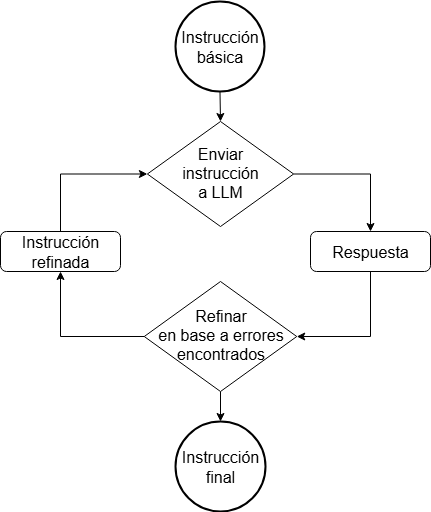
\includegraphics[width=0.7 \textwidth]{./Figures/iterative-process.png}
	\caption{Proceso de refinamiento de instrucciones.}
	\label{fig:iterativeRefinement}
\end{figure}

\pagebreak
En estre proceso se trabajó sobre cinco instrucciones diferentes:
\begin{itemize}
\item General:
se centró en resolver los problemas comunes detectados en todas las categorías narrativas.
En versiones iniciales, el modelo no generaba listas de forma adecuada ni mantenía un formato consistente en la respuesta.
También mostró dificultades para distinguir entre el contexto narrativo y las instrucciones que debía seguir.
Esto derivaba en repeticiones de información ya presentes en el texto de referencia, lo que limitaba considerablemente
la originalidad y riqueza de sus propuestas.
Por estas razones, fue necesario reformular la instrucción 
mediante la incorporación de directrices explícitas sobre el objetivo del modelo,
el formato de salida y la distinción entre contexto e instrucciones.
Se establecieron requisitos claros sobre la longitud mínima de las listas,
el nivel de detalle esperado en cada punto
y la obligatoriedad de que todos los elementos fueran completamente nuevos.
\item Eventos:
se enfocó en guiar al modelo
hacia la generación de sucesos nuevos que enriquecieran el desarrollo del mundo narrativo
sin duplicar hechos ya mencionados en el texto base.
En versiones preliminares, el modelo tendía a reformular eventos existentes en lugar de inventar situaciones originales.
Esto es debido al fuerte entrenamiento de los modelos a no modificar hechos que se consideran históricos.
Para resolver esto, se eliminó la palabra ``histórico'' de la instrucción y
se reforzó la indicación de que los eventos debían ser completamente inéditos
y conectados de forma coherente con el contexto.
\item Personajes:
las versiones iniciales del \textit{prompt} no ofrecían suficientes indicaciones estructurales,
lo que resultaba en respuestas incompletas o poco claras.
Algunos personajes carecían de nombre, contexto o motivación dentro del mundo ficticio.
Para solventar esto, la instrucción fue reescrita para exigir explícitamente un nombre, apellido,
alias (si procede) y una explicación clara de la relación del personaje con la historia o el entorno.
\item Geografía:
fue afinada para evitar confusiones entre elementos naturales y construcciones humanas.
En iteraciones anteriores, el modelo a menudo mezclaba ríos o montañas con ciudades o estructuras artificiales,
y no siempre justificaba la relevancia geográfica de los elementos descritos.
Para corregir esto, se incorporó una aclaración sobre el tipo de elementos geográficos aceptados
y se exigió una descripción detallada de cada punto, así como su importancia ecológica,
simbólica o estratégica dentro del mundo narrativo.
\item Localizaciones:
buscó mejorar la claridad y especificidad de los núcleos poblacionales propuestos.
En las versiones previas, el modelo a menudo confundía localizaciones con elementos geográficos
o entregaba descripciones genéricas sin conexión con el resto del mundo,
al utilizar la palabra ``asentamientos'' hubo una mejoría notable en el rendimiento.
La nueva versión de la instrucción estableció que debían generarse únicamente poblaciones (ciudades, pueblos, países)
y que cada una debía incluir una descripción detallada de sus características culturales, políticas o históricas,
así como su función o importancia dentro del contexto narrativo.
\end{itemize}

\pagebreak
En este proceso se utilizaron diversos corpus como contexto
con el objetivo de contrastar el comportamiento de los modelos en distintas situaciones.
A modo de anécdota, uno de los textos empleados estaba ambientado en una franquicia conocida
y los LLM generaron respuestas que incluían información propia de ese universo,
a pesar de no estar explícitamente presente en el texto proporcionado.
Esto sugiere que fueron entrenados previamente con contenidos relacionados con dicha ambientación.

Se puede consultar la versión final de las instrucciones desarrolladas en este trabajo en el apéndice \ref{AppendixA}.
Dado que el inglés es el idioma preferente de los modelos,
las instrucciones se redactaron en ese idioma.
Por esto mismo, se incluye una instrucción final para que la respuesta se genere en el idioma seleccionado por el usuario.
Sin embargo, es importante señalar que no todos los modelos soportan el español,
lo que ocasionalmente lleva a que esta última instrucción sea ignorada.
Este fenómeno se detallará en la siguiente sección.